\chapter{Evaluation}
This chapter provides an insight into the data collected from the questionnaires and the feedback system logs while also explaining results derived from statistical tests. The chapter is structured as follows: \S\ref{sec:eval-demographic} provides an over of the demographic background for the sampled participants. \S\ref{sec:eval-distTests} covers test which check the data sets distribution moving on to compare the distribution across the feedback group and base group. \S\ref{sec:eval-feedbackSysResults} goes through determining any difference between the two groups which might have been cuased by the introduction of the feedback system.  \S\ref{sec:eval-usersFeedback} covers the participants impressions on the experiment and finally conclusive results from this study are presented in \S\ref{sec:eval-Discussion} 

\begin{figure}
	\centering
	\begin{minipage}{0.45\textwidth}
		\centering
		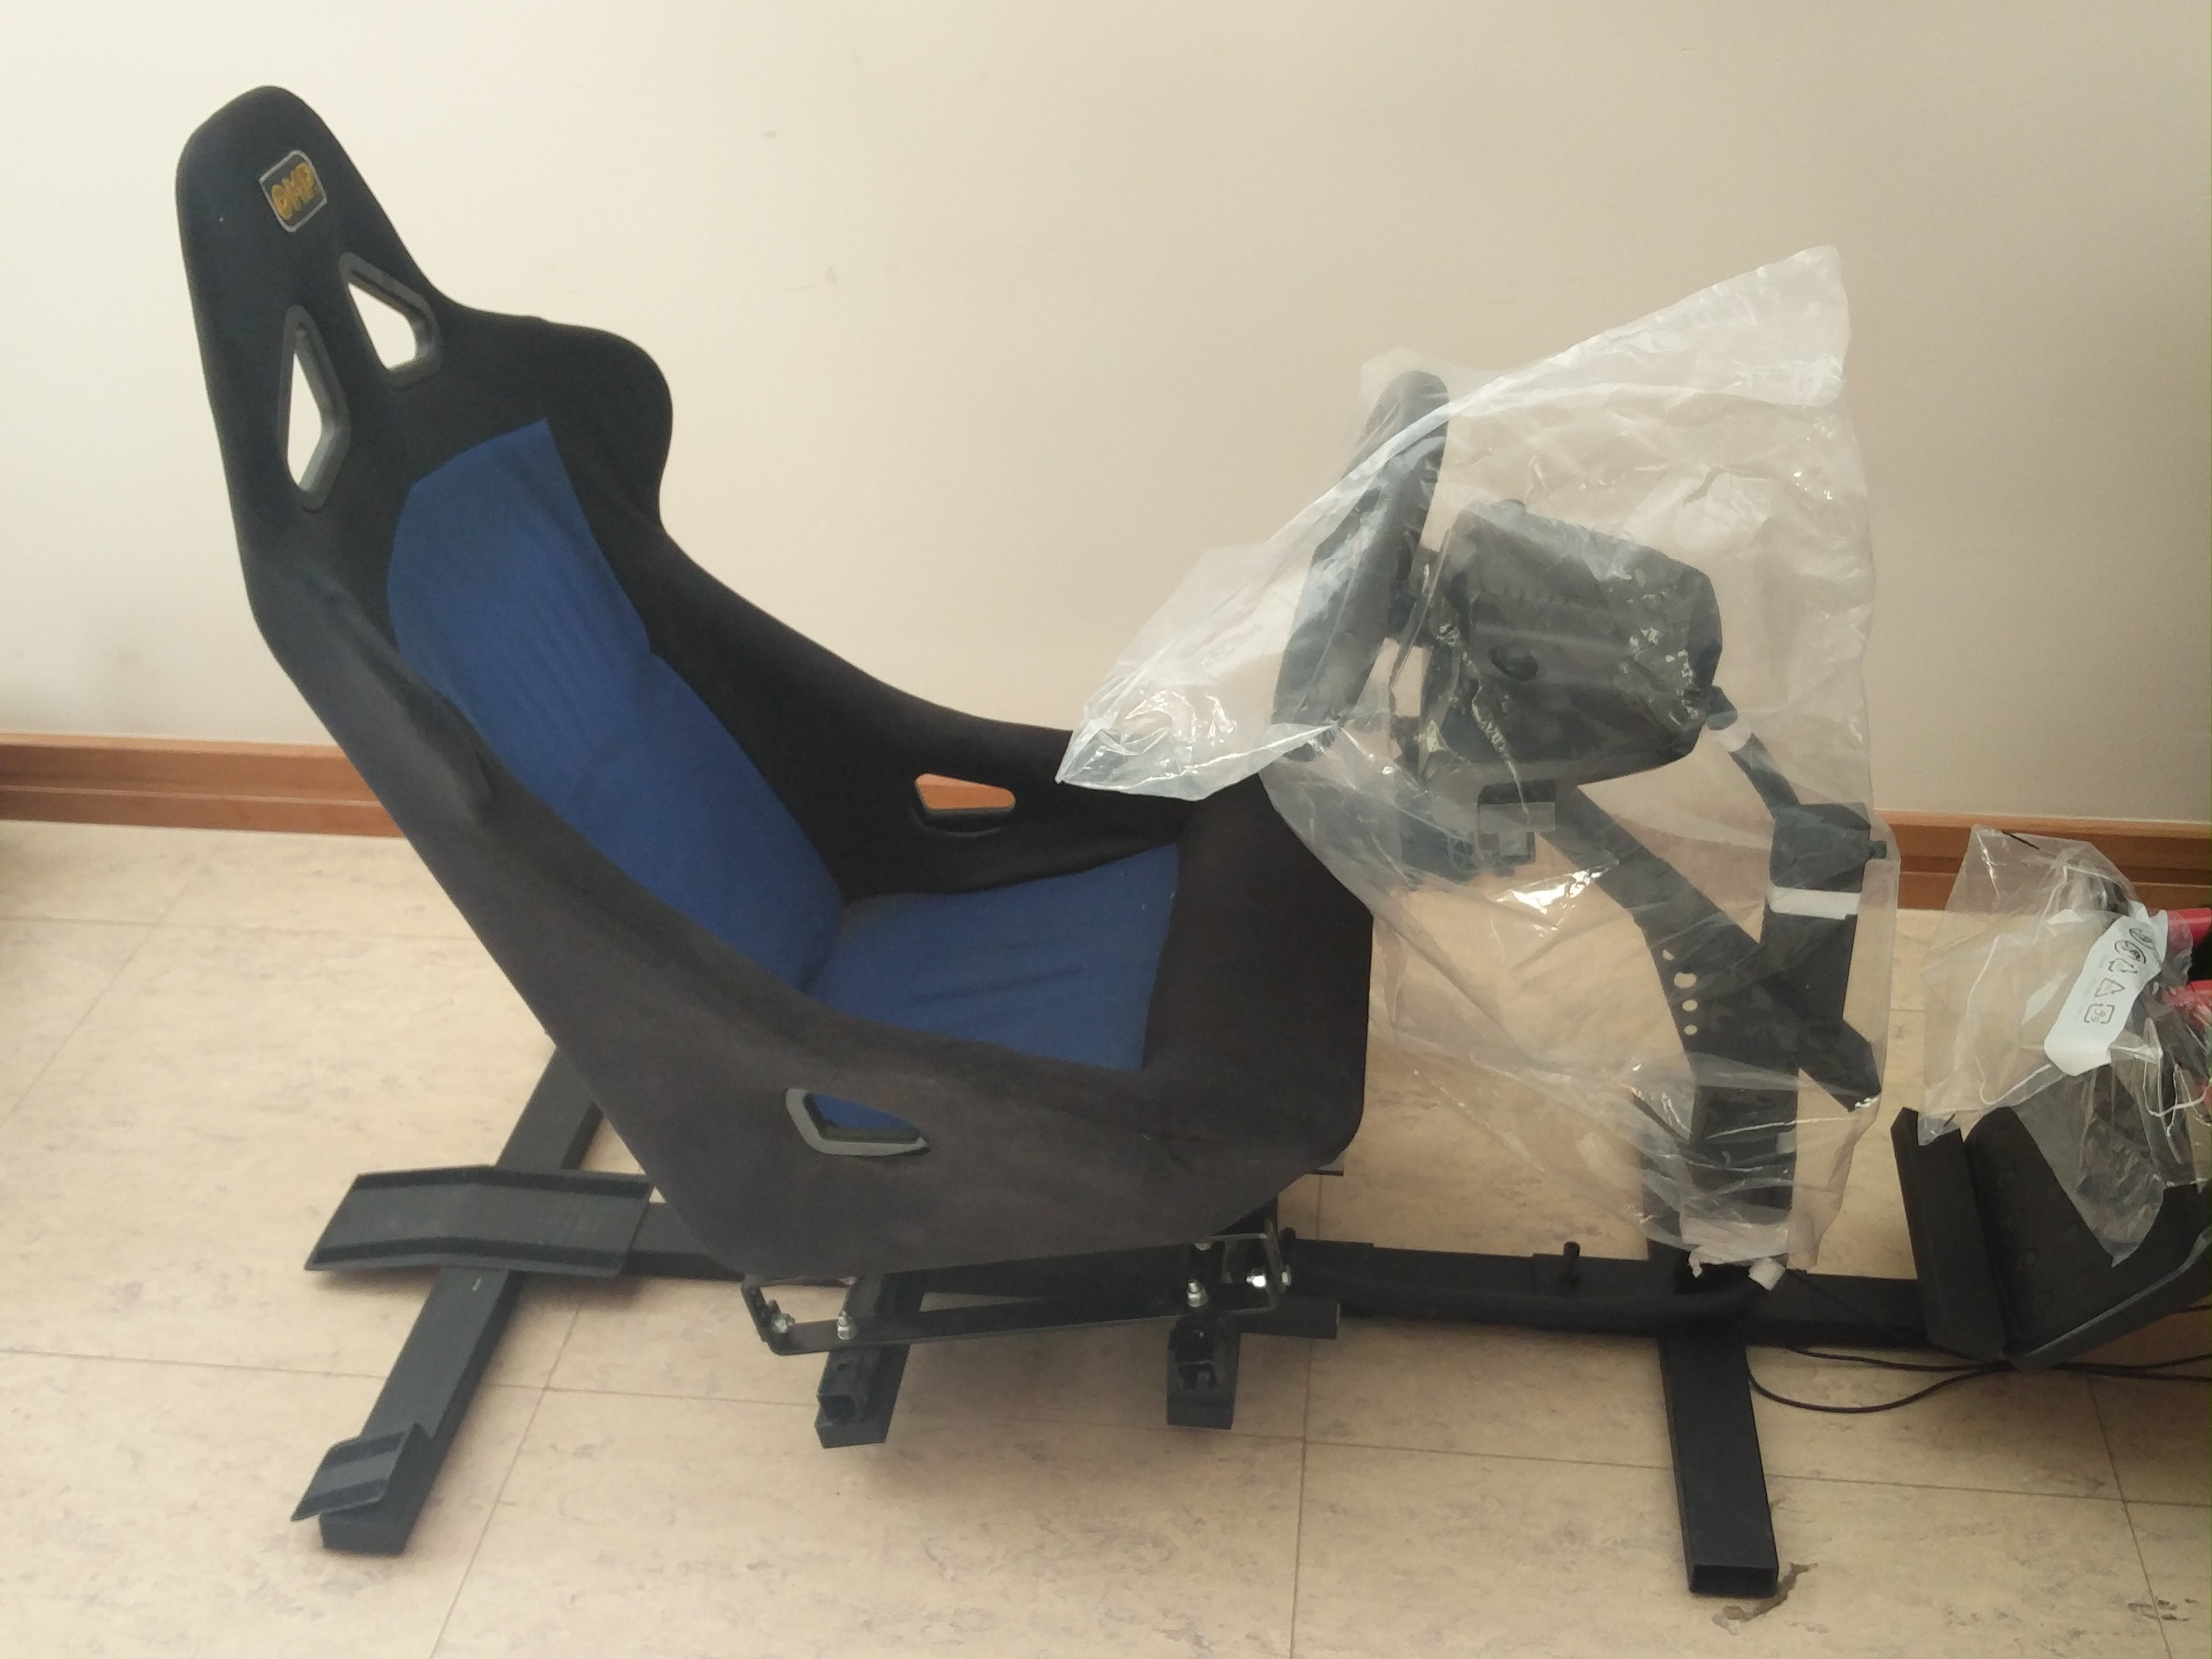
\includegraphics[width=\textwidth]{images/RacingRig}
		\caption{Side view of the racing rig}
	\end{minipage}\hfill
	\begin{minipage}{0.45\textwidth}
		\centering
		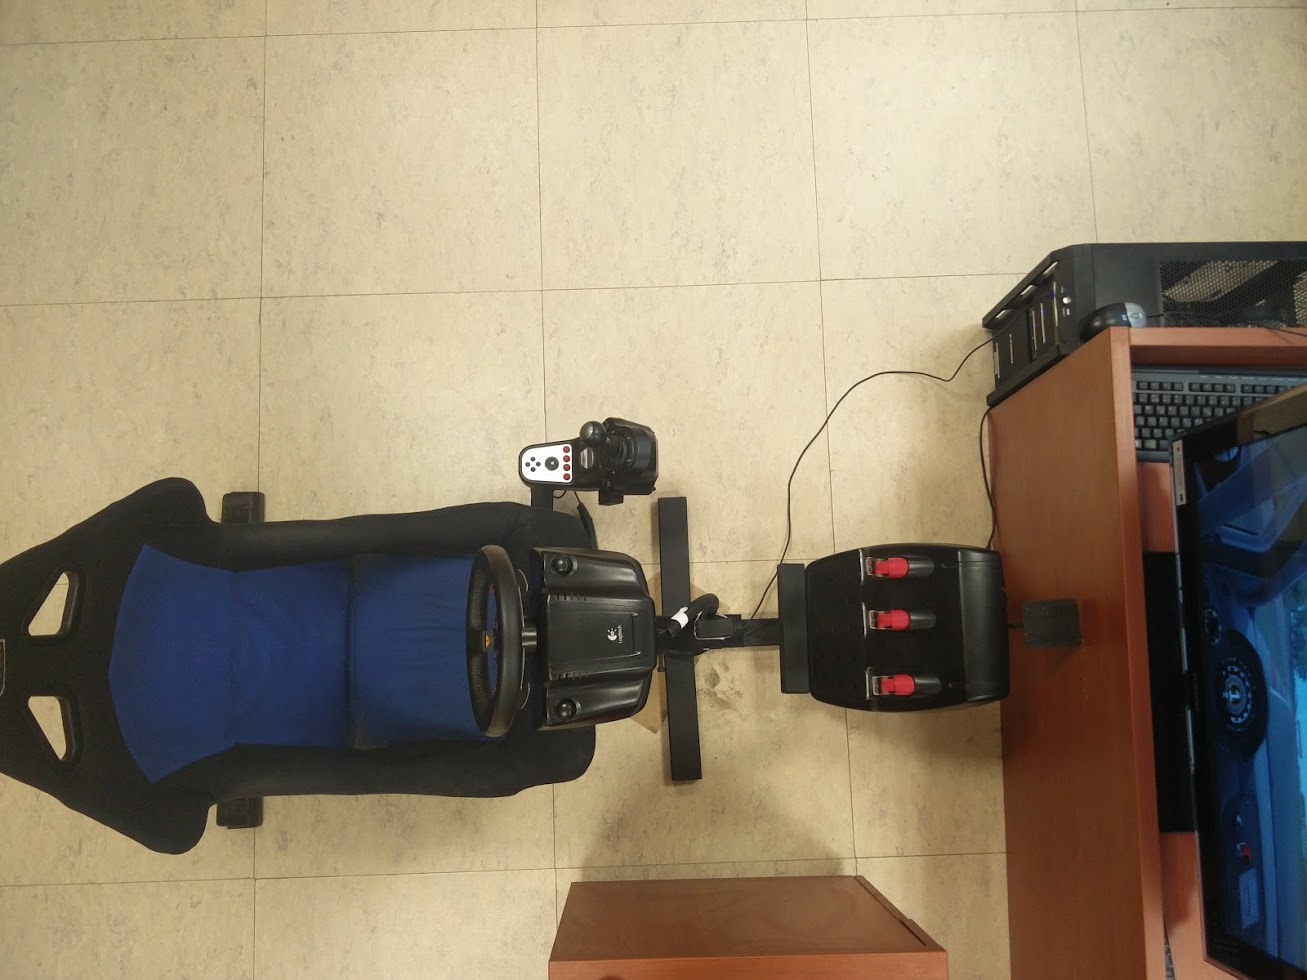
\includegraphics[width=\textwidth]{images/RacingRig2}
		\caption{Top view of the racing rig}
	\end{minipage}
\end{figure}

\section{Experiment Setup}
\label{sec:imp-simRacingRig}
Link back to methodology using Chapter \ref{chp:methodology}.
Display model and make, PC configuration. 

%The rig is made out of various independent components. The steering wheel is a Logitech G25 a pedal set, an H shifter and a bucket racing seat, all mounted on to a home made metal frame.

\begin{figure}[!htb]
	\centering
	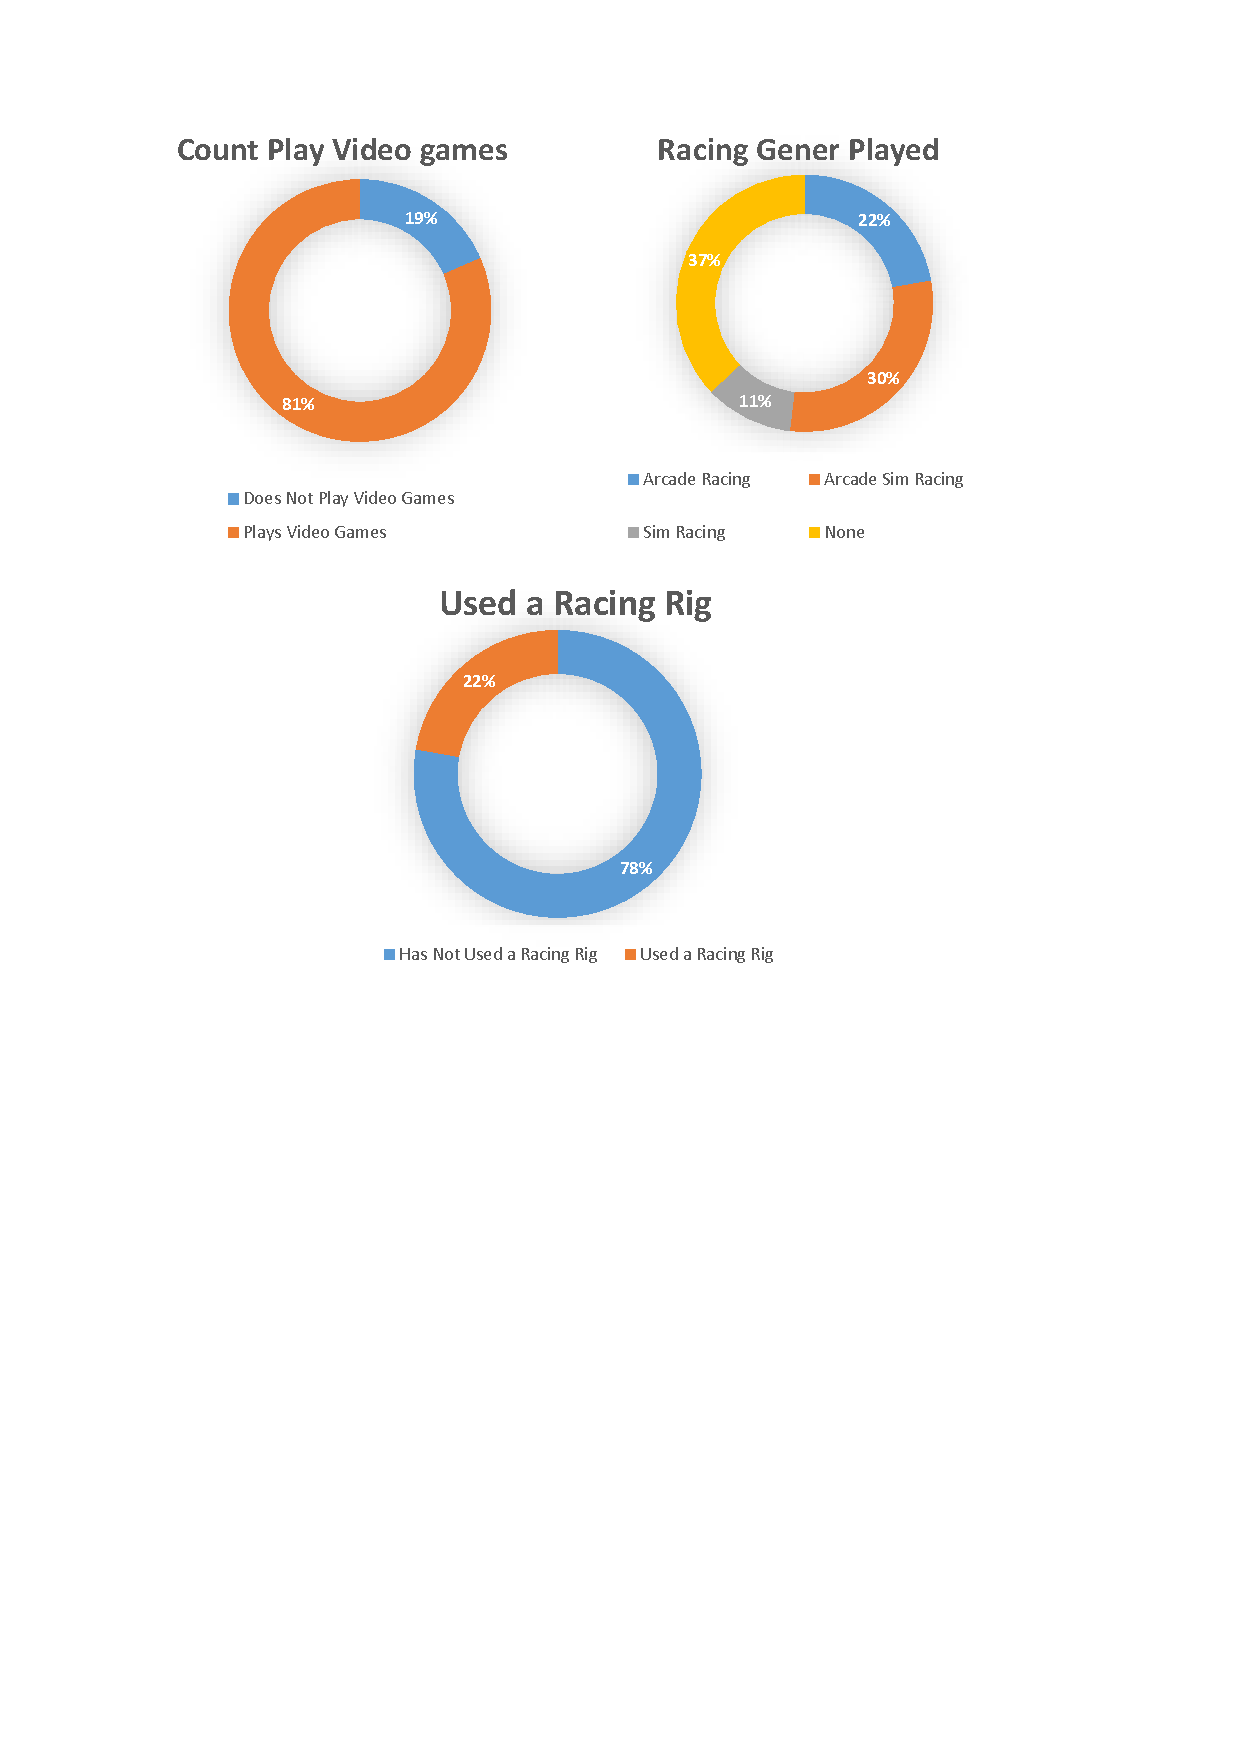
\includegraphics[height=10cm]{charts/gamesxp.pdf}
	\caption[Gaming xp]{Video games experience}
	\label{fig:chart-gamesxp}
\end{figure}

\section{Sample Demographic}
\label{sec:eval-demographic}

The following demographic data was drawn out from the pre study survey. Participant's were mostly in their early twenties and mostly males. Out of 27 participants, 2 didn't have a driving license and 25 had a driving license with most of them have been driving for a year. Furthermore 22 participants identified them self as playing videos games, from which 18 participants stated they have played racing video games. The majority of participants who plays racing games identified them self as playing mostly arcade sim racing games, while only 3 play sim racing games. Out of the 27 participants, 7 participants have previously used a racing rig. 

\emph{Mention the sample split between each group (control/feedback).}

%I included the charts in the appendices as I didn't feel like they were adding much over here ending up just taking space.

\begin{figure}[!htb]
	\centering
	\includegraphics[width=\textwidth]{charts/laptimes.png}
	\caption{Lap times vs session, clustered by group}
	\label{fig:chart-laptimes}
\end{figure}

\section{Distribution Tests}
\label{sec:eval-distTests}
\emph{Explain p-values wrt confidence interval and the specific values you are aiming for.}

From the lap times box plot \ref{xxx}, one can notice a trend in which lap times improve the more time they use the rig, irrespective of the group assignment. It's worth pointing out the median of the feedback group is lower than the base group's median, except during the last session in which the medians are close to each other. Moreover the participants in the feedback group seem to be less consistent in their lap times as the box plot whiskers and quartiles are more spread out then the ones from the base group.

Carrying out Shapiro-Wilk test for normality for the feedback group and base group during the first session on their respective lap times it was found that the data is not normally distributed as the p-value for both groups is below 0.05 resulting in rejecting the null hypothesis stating the samples come from a normal distribution.

\begin{figure}[!htb]
	\centering
	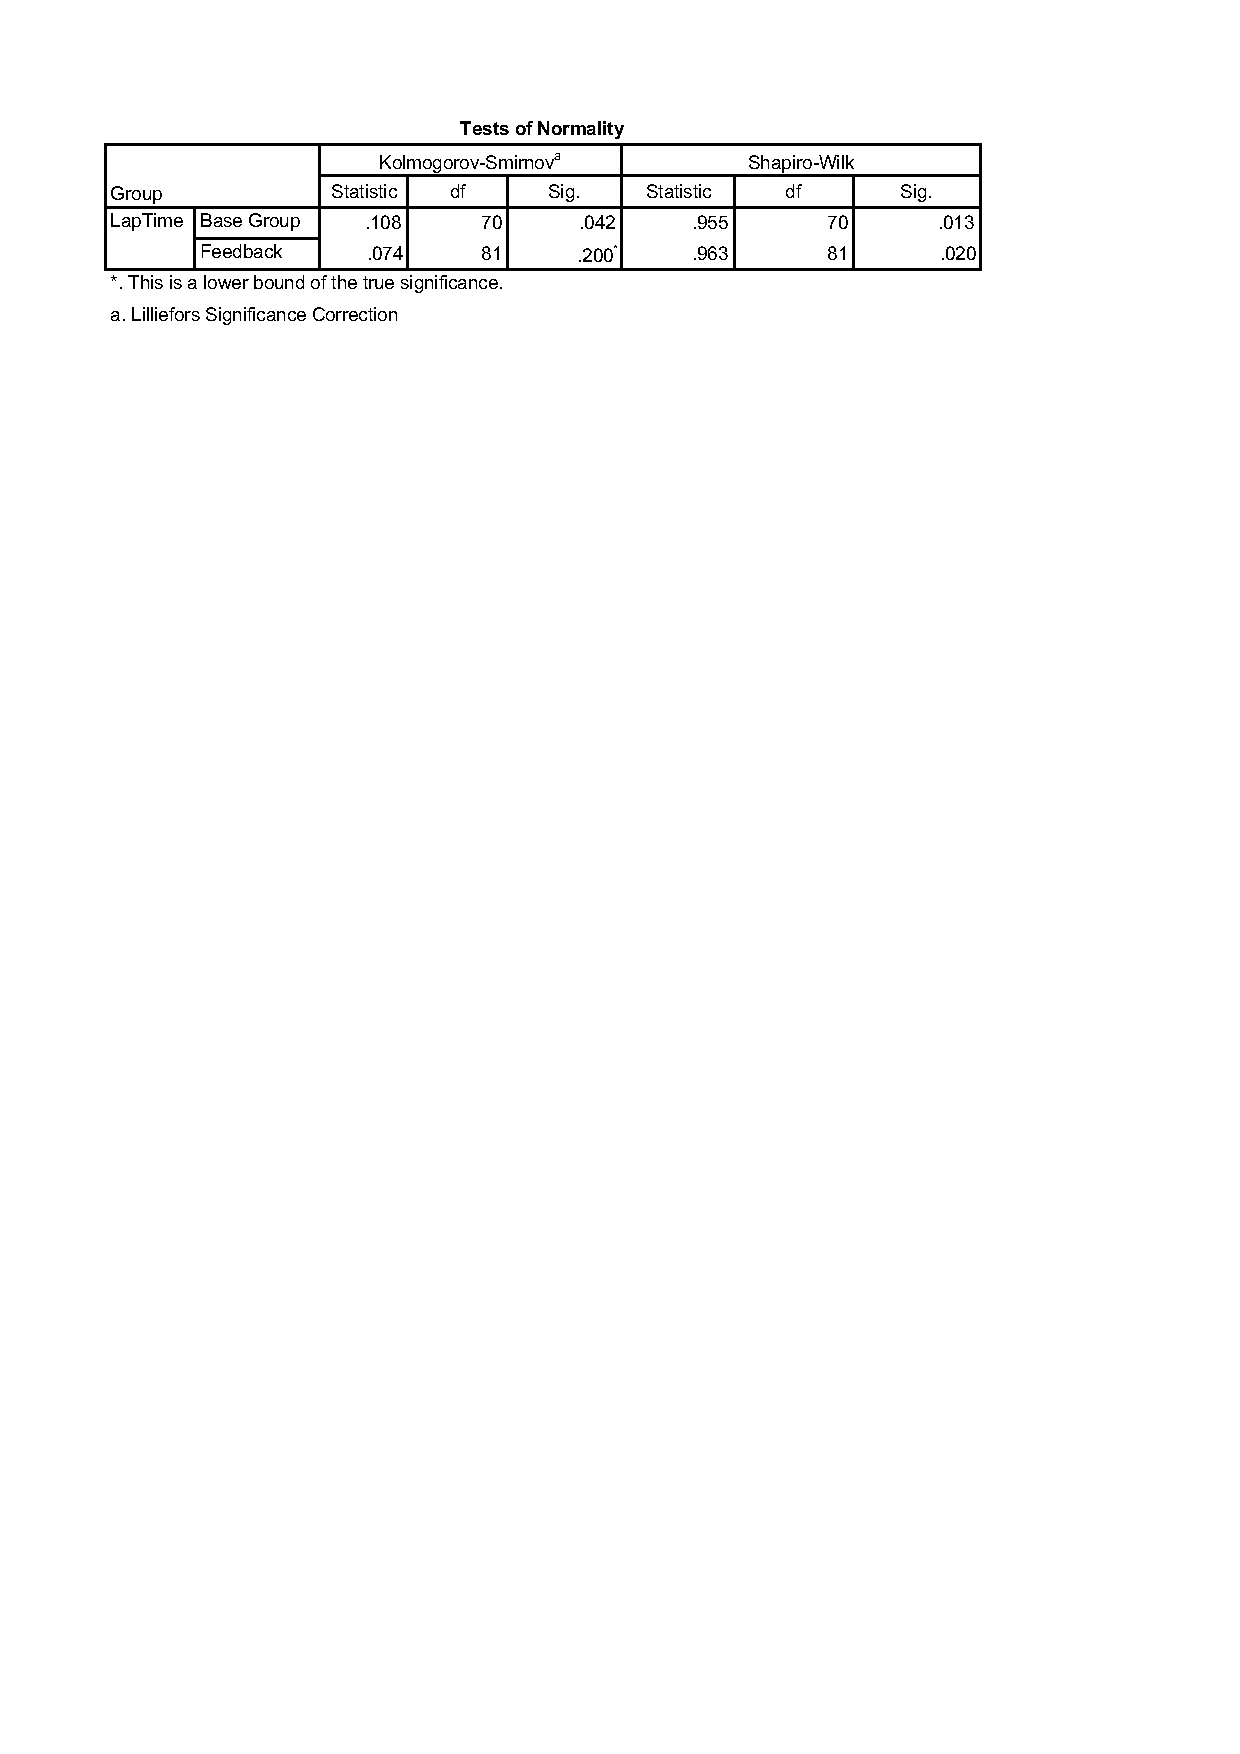
\includegraphics[width=\textwidth]{charts/shapiroWilkResults.pdf}
	\caption[Shapiro Wilk]{Shapiro Wilk test results}
	\label{fig:chart-shapiroWilk}
\end{figure}

The same data was checked for similar distribution across groups using the Kolmogorov-Smirnov Test which resulted in accepting the null hypothesis stating the groups' lap times share the same distribution.

\begin{figure}[!htb]
	\centering
	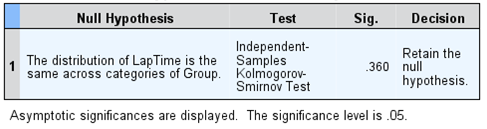
\includegraphics[width=\textwidth]{images/KolmogorowSmimov.png}
	\caption[Kolmogorow Smimov Test]{Kolmogorow Smimov test result}
	\label{fig:chart-KolmogorowSmimov}
\end{figure}

\section{Feedback System Results}
\label{sec:eval-feedbackSysResults}
Having established both groups' lap times share the same distribution during the first session the Mann-Whitney Test to determine any differences between the groups before the feedback system is introduced. The test results show a p value of 0.057 resulting in no statistical difference between the groups at the start of the sessions.

\begin{figure}[!htb]
	\centering
	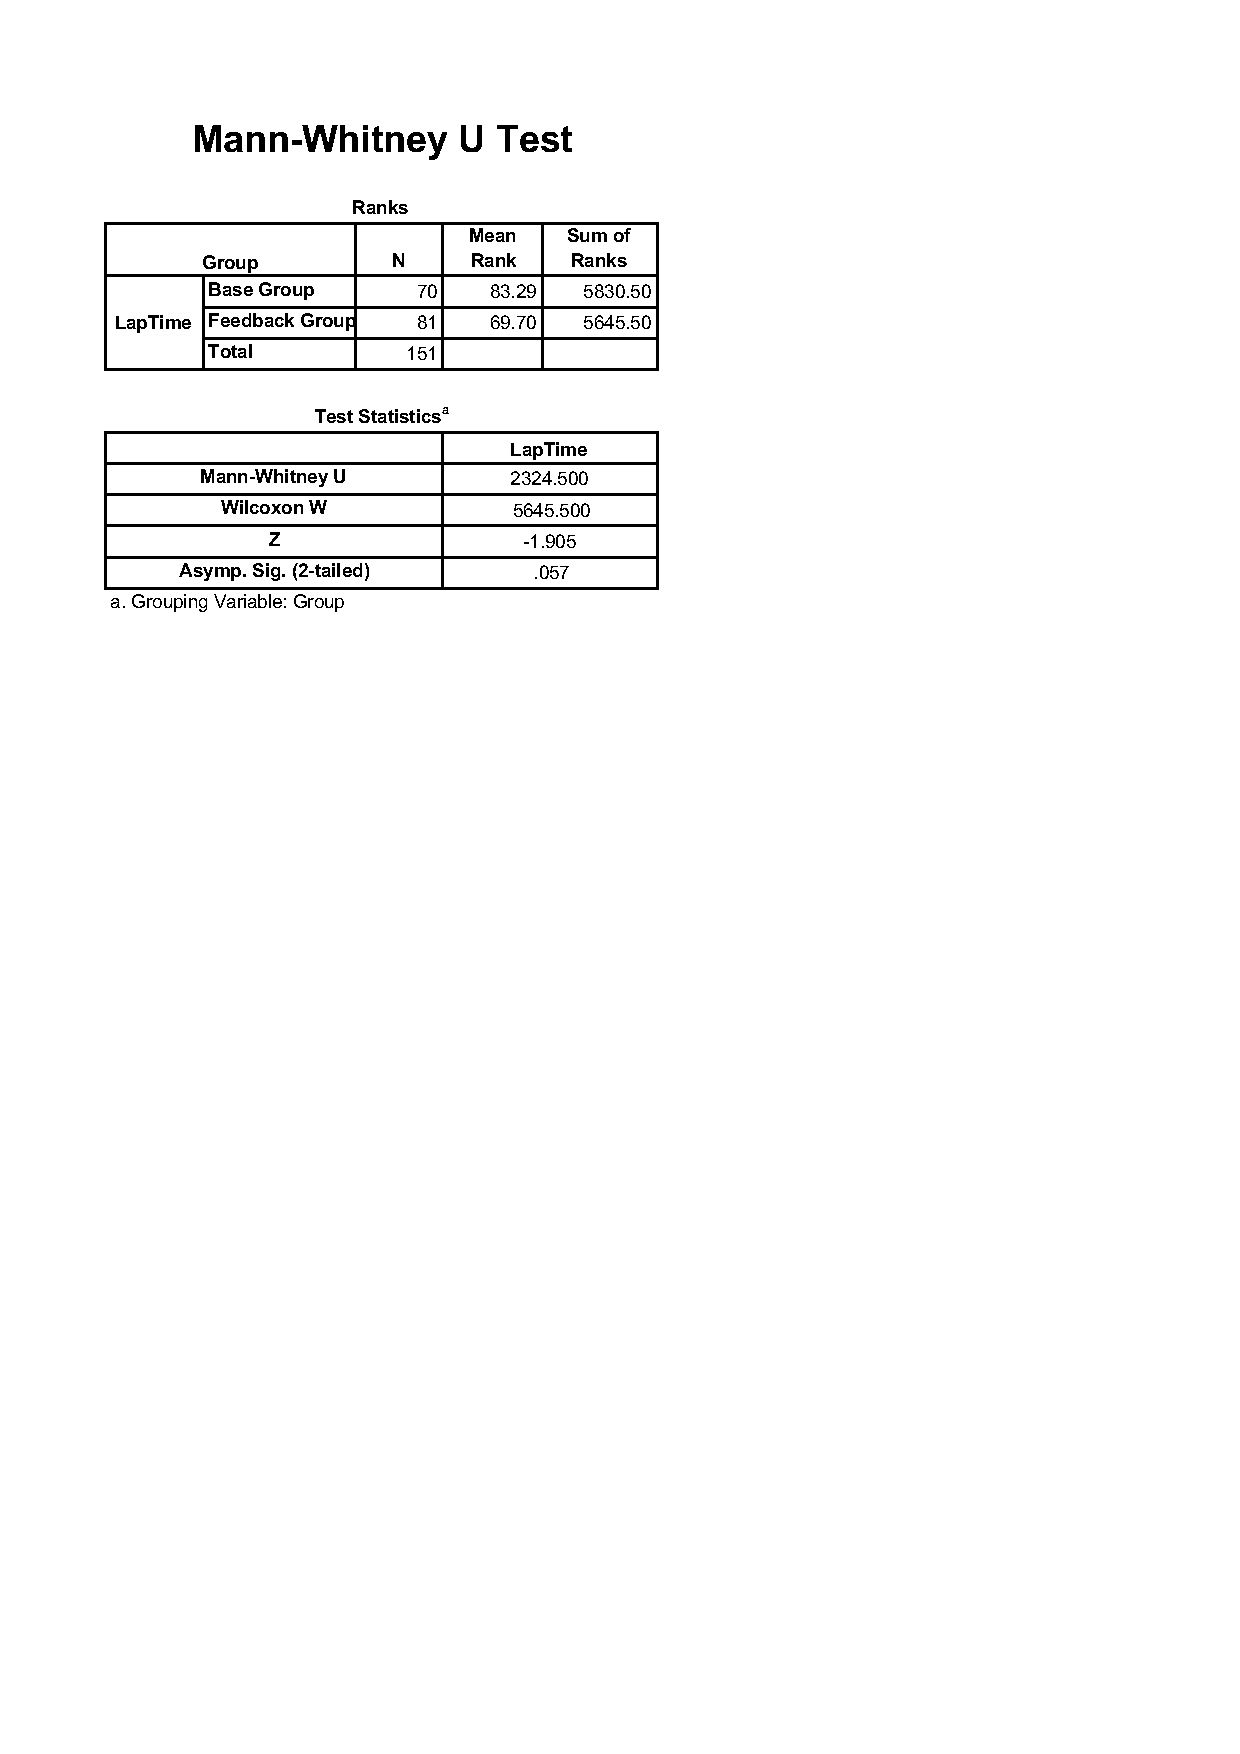
\includegraphics[width=\textwidth]{charts/Mann-Whitney.pdf}
	\caption[Mann-Whitney]{Mann-Whitney Test results}
	\label{fig:chart-KolmogorowSmimov}
\end{figure}

Running the Mann-Whitney Test on the remaining sessions, results show there is no significant difference between the two groups even after the feedback system was introduced to one group. The third session tells a different story as the p-value is 0.029 which results is accepting the null hypothesis. The fourth and final sessions is the one which both groups had the feedback system turned off which resulted in the difference between the groups to yet again show no statistical significant difference.

\begin{figure}[!htb]
	\centering
	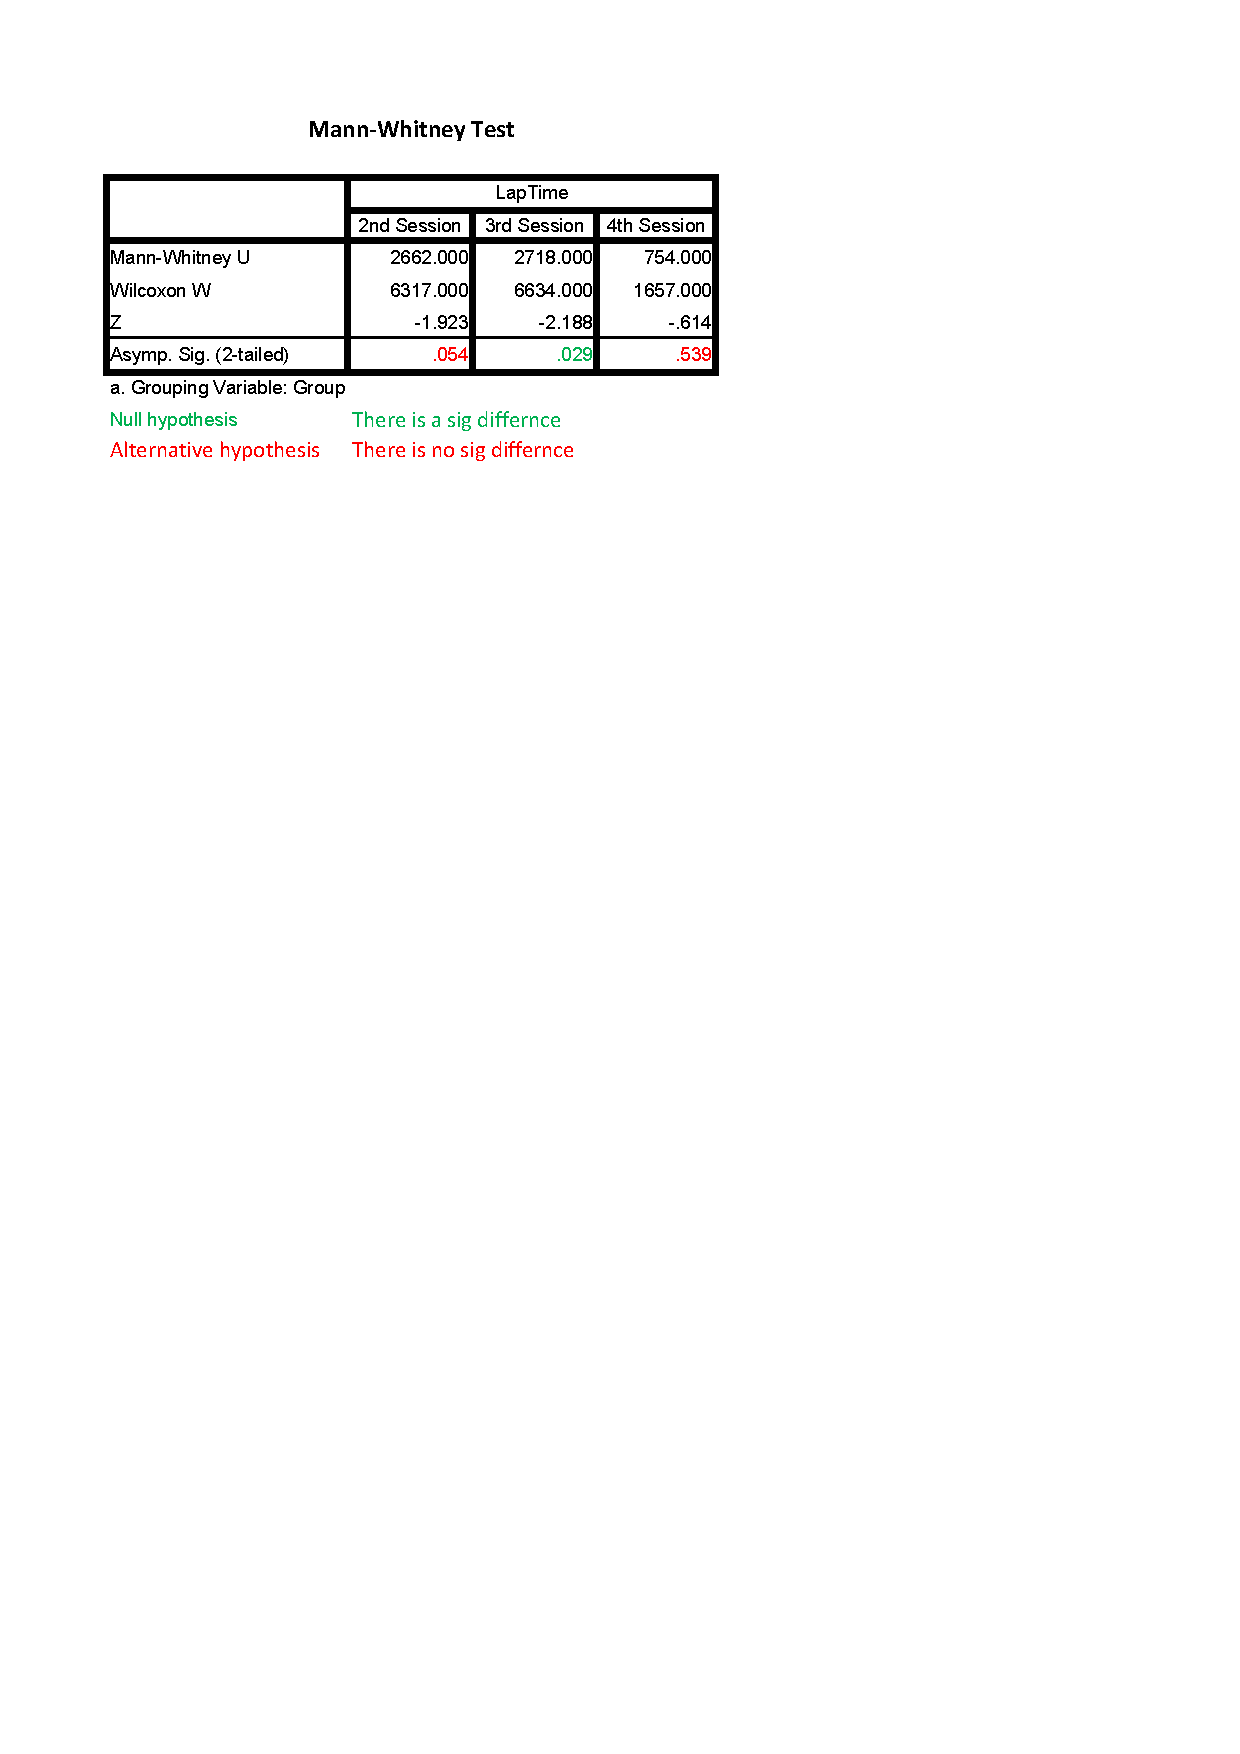
\includegraphics[width=\textwidth]{charts/Mann-Whitney-Sessions.pdf}
	\caption[Mann-Whitney Accross Sessions]{Mann-Whitney test result for the last the sessions}
	\label{fig:chart-Mann-Whitney-Sessions}
\end{figure}

\section{Participant Feedback}
\label{sec:eval-usersFeedback}
Participants reported an overall good experience, the rig setup was found to be realistic and easy to use. An overwhelming majority of the participants reported having issues mastering the s-bend part of the track, however, they reported that the car and track choice was an adequate one. When the feedback group was asked about the feedback system, they reported to be intelligible, accurate, helpful and somewhat easy to apply the feedback given. Lastly, when asked about if the thought the feedback was intrusive, possible distracting them, out of 15, 5 reported it to be intrusive.

\begin{figure}[!htb]
	\centering
	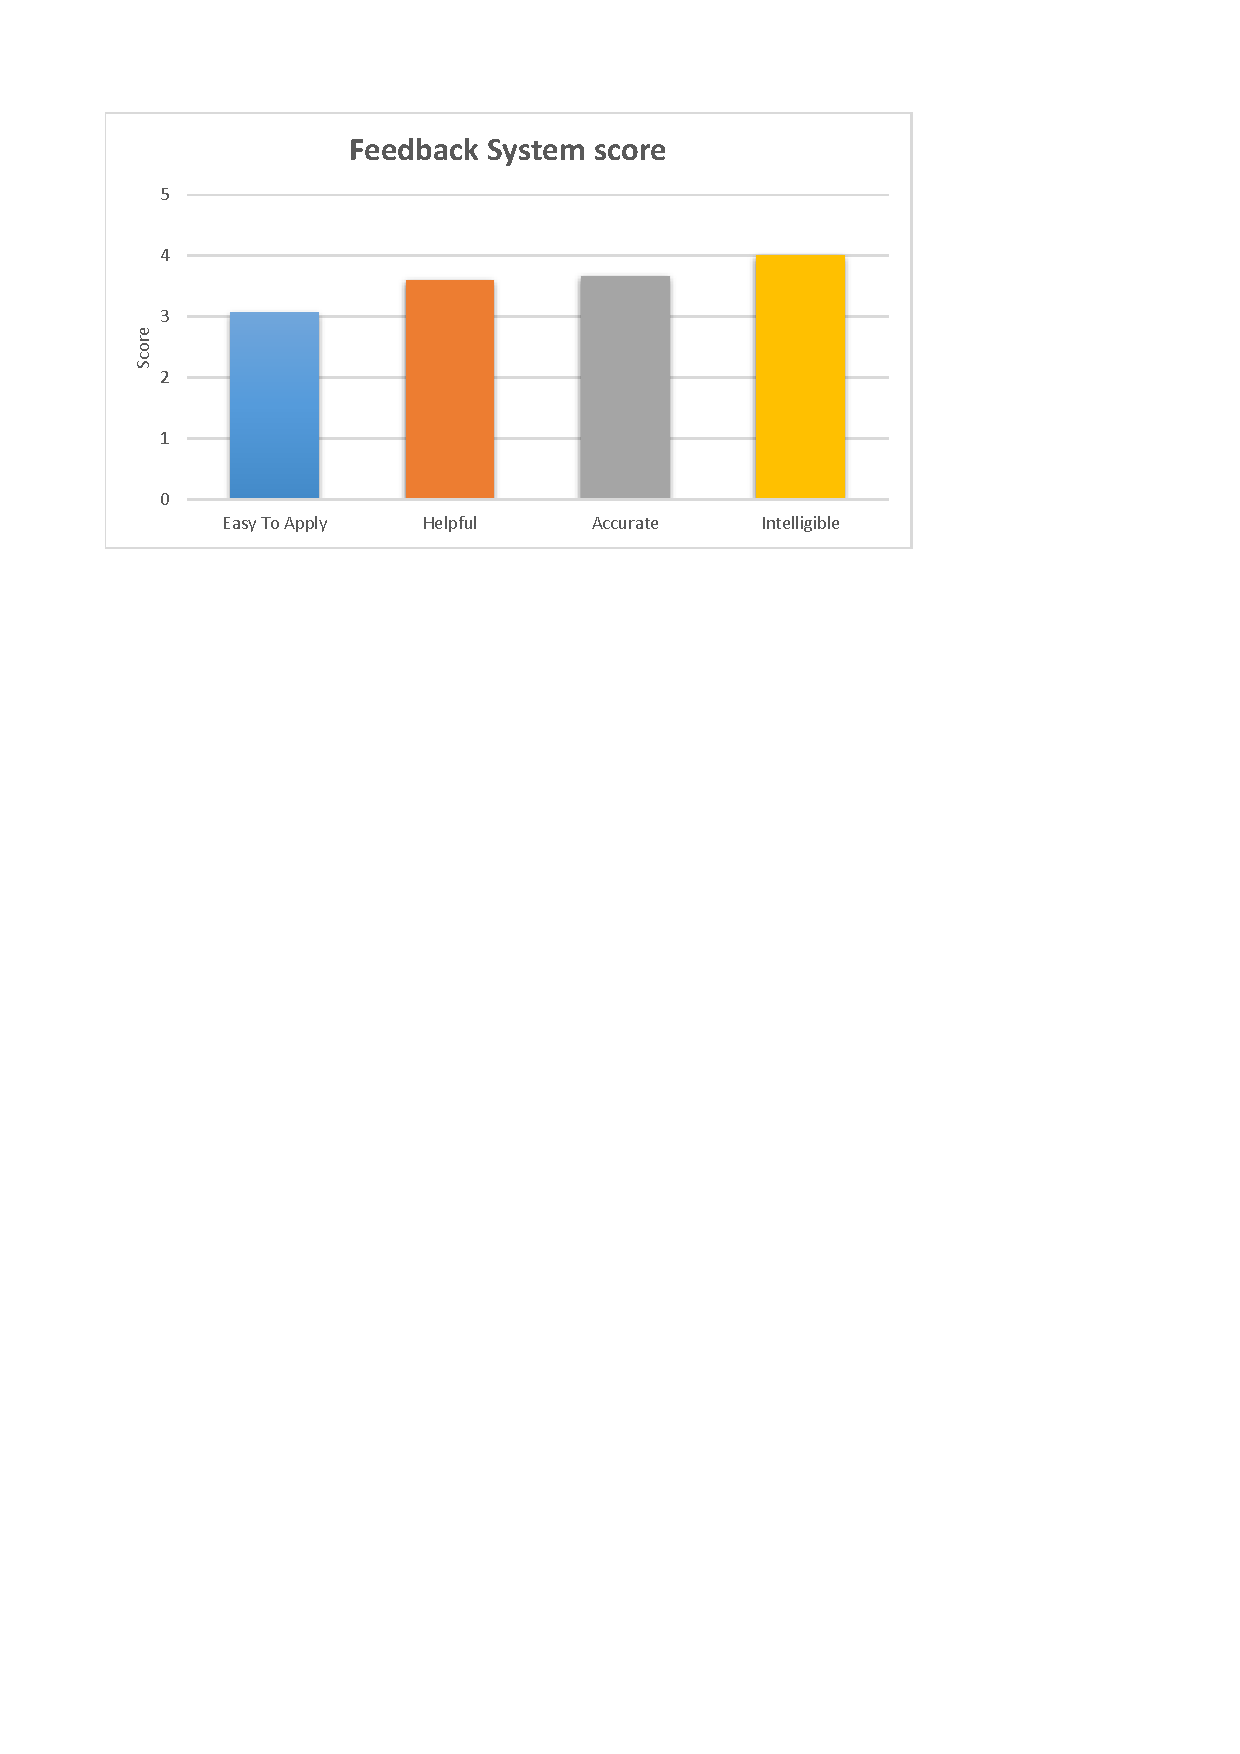
\includegraphics[width=\textwidth]{charts/feedbacksystemfeedback.pdf}
	\caption[Participants' Feedback]{Participants' Feedback}
	\label{fig:chart-feedbacksystemfeedback}
\end{figure}

\section{Discussion}
\label{sec:eval-Discussion}
From the post experiment questionnaire one can note that rig setup has been well received, with participants enjoying the experiments while also given it a high score for it sense of realism. This suggests that by using off the shelf entry level hardware for the sim racing rig, it is possible to achieve a good level of realism. the feedback system shows to have potential. the groups start of the same skill level. Both groups show a noticeable improvement from one session to the next session, excluding the last session in which it seems the shorter session might have put extra pressure on the participants' hindering their performance. Furthermore there was not statistical difference during the second session, but during the third session there was. The fact that the feedback group had a lower average lap time it suggest the group managed to get used to the feedback system after the second session and start to follow the feedback instructions during the third session. Lastly the sample is too simple to test for correlation between gaming experience and lap times, as only two players have played sim racing games while the other gamers don't play enough racing games. Same goes for correlation between having a driving licences and being able to the user the rig, as only two unlicensed participants took part, both of which are in the process of obtaining their driving license.

\section{Summary}